\documentclass{article}

\usepackage{multicol}
\usepackage{lipsum}
\usepackage{graphicx}
\graphicspath{{images/}}
\usepackage{blindtext}
\usepackage{subfiles} % Best loaded last in the preamble
\usepackage[dvipsnames]{xcolor}
\usepackage[T1]{fontenc}
\usepackage{setspace}
\usepackage{float}

\setlength{\columnsep}{1cm}

\usepackage{fullpage, tikz}
\usepackage{eso-pic}
\AddToShipoutPictureBG{%
	\begin{tikzpicture}[remember picture, overlay]
		\node[opacity=.4, inner sep=0pt]
		at(current page.center){
\includegraphics[width=8.5in, height=11in]{images/background}};
	\end{tikzpicture}%
}

\usepackage[margin={1.5cm,1.5cm}]{geometry}

\newcommand\BackgroundPic{%
	\put(0,0){%
		\parbox[b][\paperheight]{\paperwidth}{%
			\vfill
			\centering
			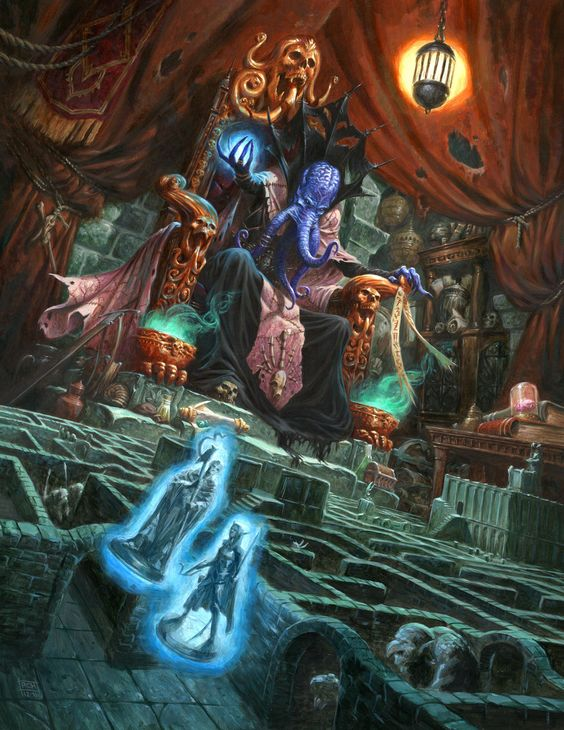
\includegraphics[width=\paperwidth,height=\paperheight]{images/cover.jpg}%
			\vfill
}}}

\title{\color{white}\textsc{\Huge Mystery at Valboro Observatory }}
\date{ }


\setlength\fboxsep{8pt}

\begin{document}
	\AddToShipoutPicture*{\BackgroundPic}
	\maketitle
	\pagebreak
	\begin{multicols*}{2}
	\section{Introduction}
	
		\subsection*{Overview}
		The \emph{Mystery at Valboro Observatory} one-off adventures is meant to be played with a group of NUMPLAYERS players at level PLAYERLEVEL. The adventure is meant to be completed in one session.
		
		The setting for the story is at the Valboro Observatory, on the island of Valboro. A rare astrological event has caused a time rift to open, which is being amplified by the ancient telescope built directly through the mountain. On the other side of the rift, a mysterious figure known as the \emph{Time Harvester} has been using this event to collect and convert time itself as energy.
		
		Time within the observatory itself is at an almost standstill, and once the players find themselves within it, there is no escape from it. The only escape is to breach the rift and defeat the \emph{Time Harvester}.
		
		\subsection*{Background}
		The heroes find themselves on the island of Valboro, known for it's beautiful weather, wealth and vineyards from which is produced the finest quality wine in the know world. The group has been hired by the Winemakers Guild to investigate mysterious circumstances around the famous Valboro Observatory.
		
		The Valboro Observatory is critically important to Valborian society and to the Winemakers Guild because it provides very sophisticated weekly weather reports which contain essential information useful for the local agriculture and wine-making process. The observatory is centuries old and was originally built by brilliant gnomish engineers and scientists, who still operate it to this day. 
		
		The headmaster of the observatory is an older gnome named Frunsmag Karn. The scientists working at the observatory study various meteorological and astronomical sciences to produce finely tuned weekly weather predictions which helps local agriculture and vineyards. The gnomes have owned and operated the observatory for centuries and their trade has been passed down for many generations, making it the most sophisticated weather prediction in the known world.
		
		The observatory is located high up in the Boro mountains, about a three days journey north-west of the coastal capital city of Aleytheas. Built right into the side of a large mountain, it is a marvel of modern engineering and architecture. It is a large cylindrical structure with a domed top containing the main telescope.
		
		\subsection*{Quest}
		For the past month, the Winemakers Guild have grown concerned over the lack of reports or information from the observatory. The Guild sent the Valborian Guard and other mercenaries to investigate but none have returned in weeks. Desperate for this situation to be resolved, the Guild decided to hire off-islander heroes to discover what has transpired at the observatory. The heroes must hurry as every day that passes by without reports is damaging to local farmers and winemakers. The heroes will be handsomely rewarded with a sum of \textbf{10,000 gp} by the Guild for their success.
		
		As the sun sets over the mountains, the adventure begins with the players arriving at the observatory, only to find it eerily abandoned...
		
	\section{The Valboro Observatory}
		Arriving at the observatory, the players stand in front of a long staircase leading to the main entrance to the cylindrical shaped structure. Various broken or abandoned weather measuring devices litter the area around the observatory. The players may choose to investigate the area but there's nothing of value to be found. Since it is built right on the side of the mountain, the terrain around it is extremely treacherous, so there doesn't appear to be any other entrances to the observatory.
		
		The heroes should make their way up the stairs and to the main entrance, which consists of very large and heavy metal doors. The doors are designed to close back up by themselves; once all of the players have passed through the door, they are now trapped in the observatory. 
		
		The air in the observatory smells stale and musty, with a faint smell of death and decay. A quiet humming noise from the generator can be heard, causing the lights to buzz and flicker quickly in the dimly lit rooms.
		
		\begin{figure*}
			\centering
			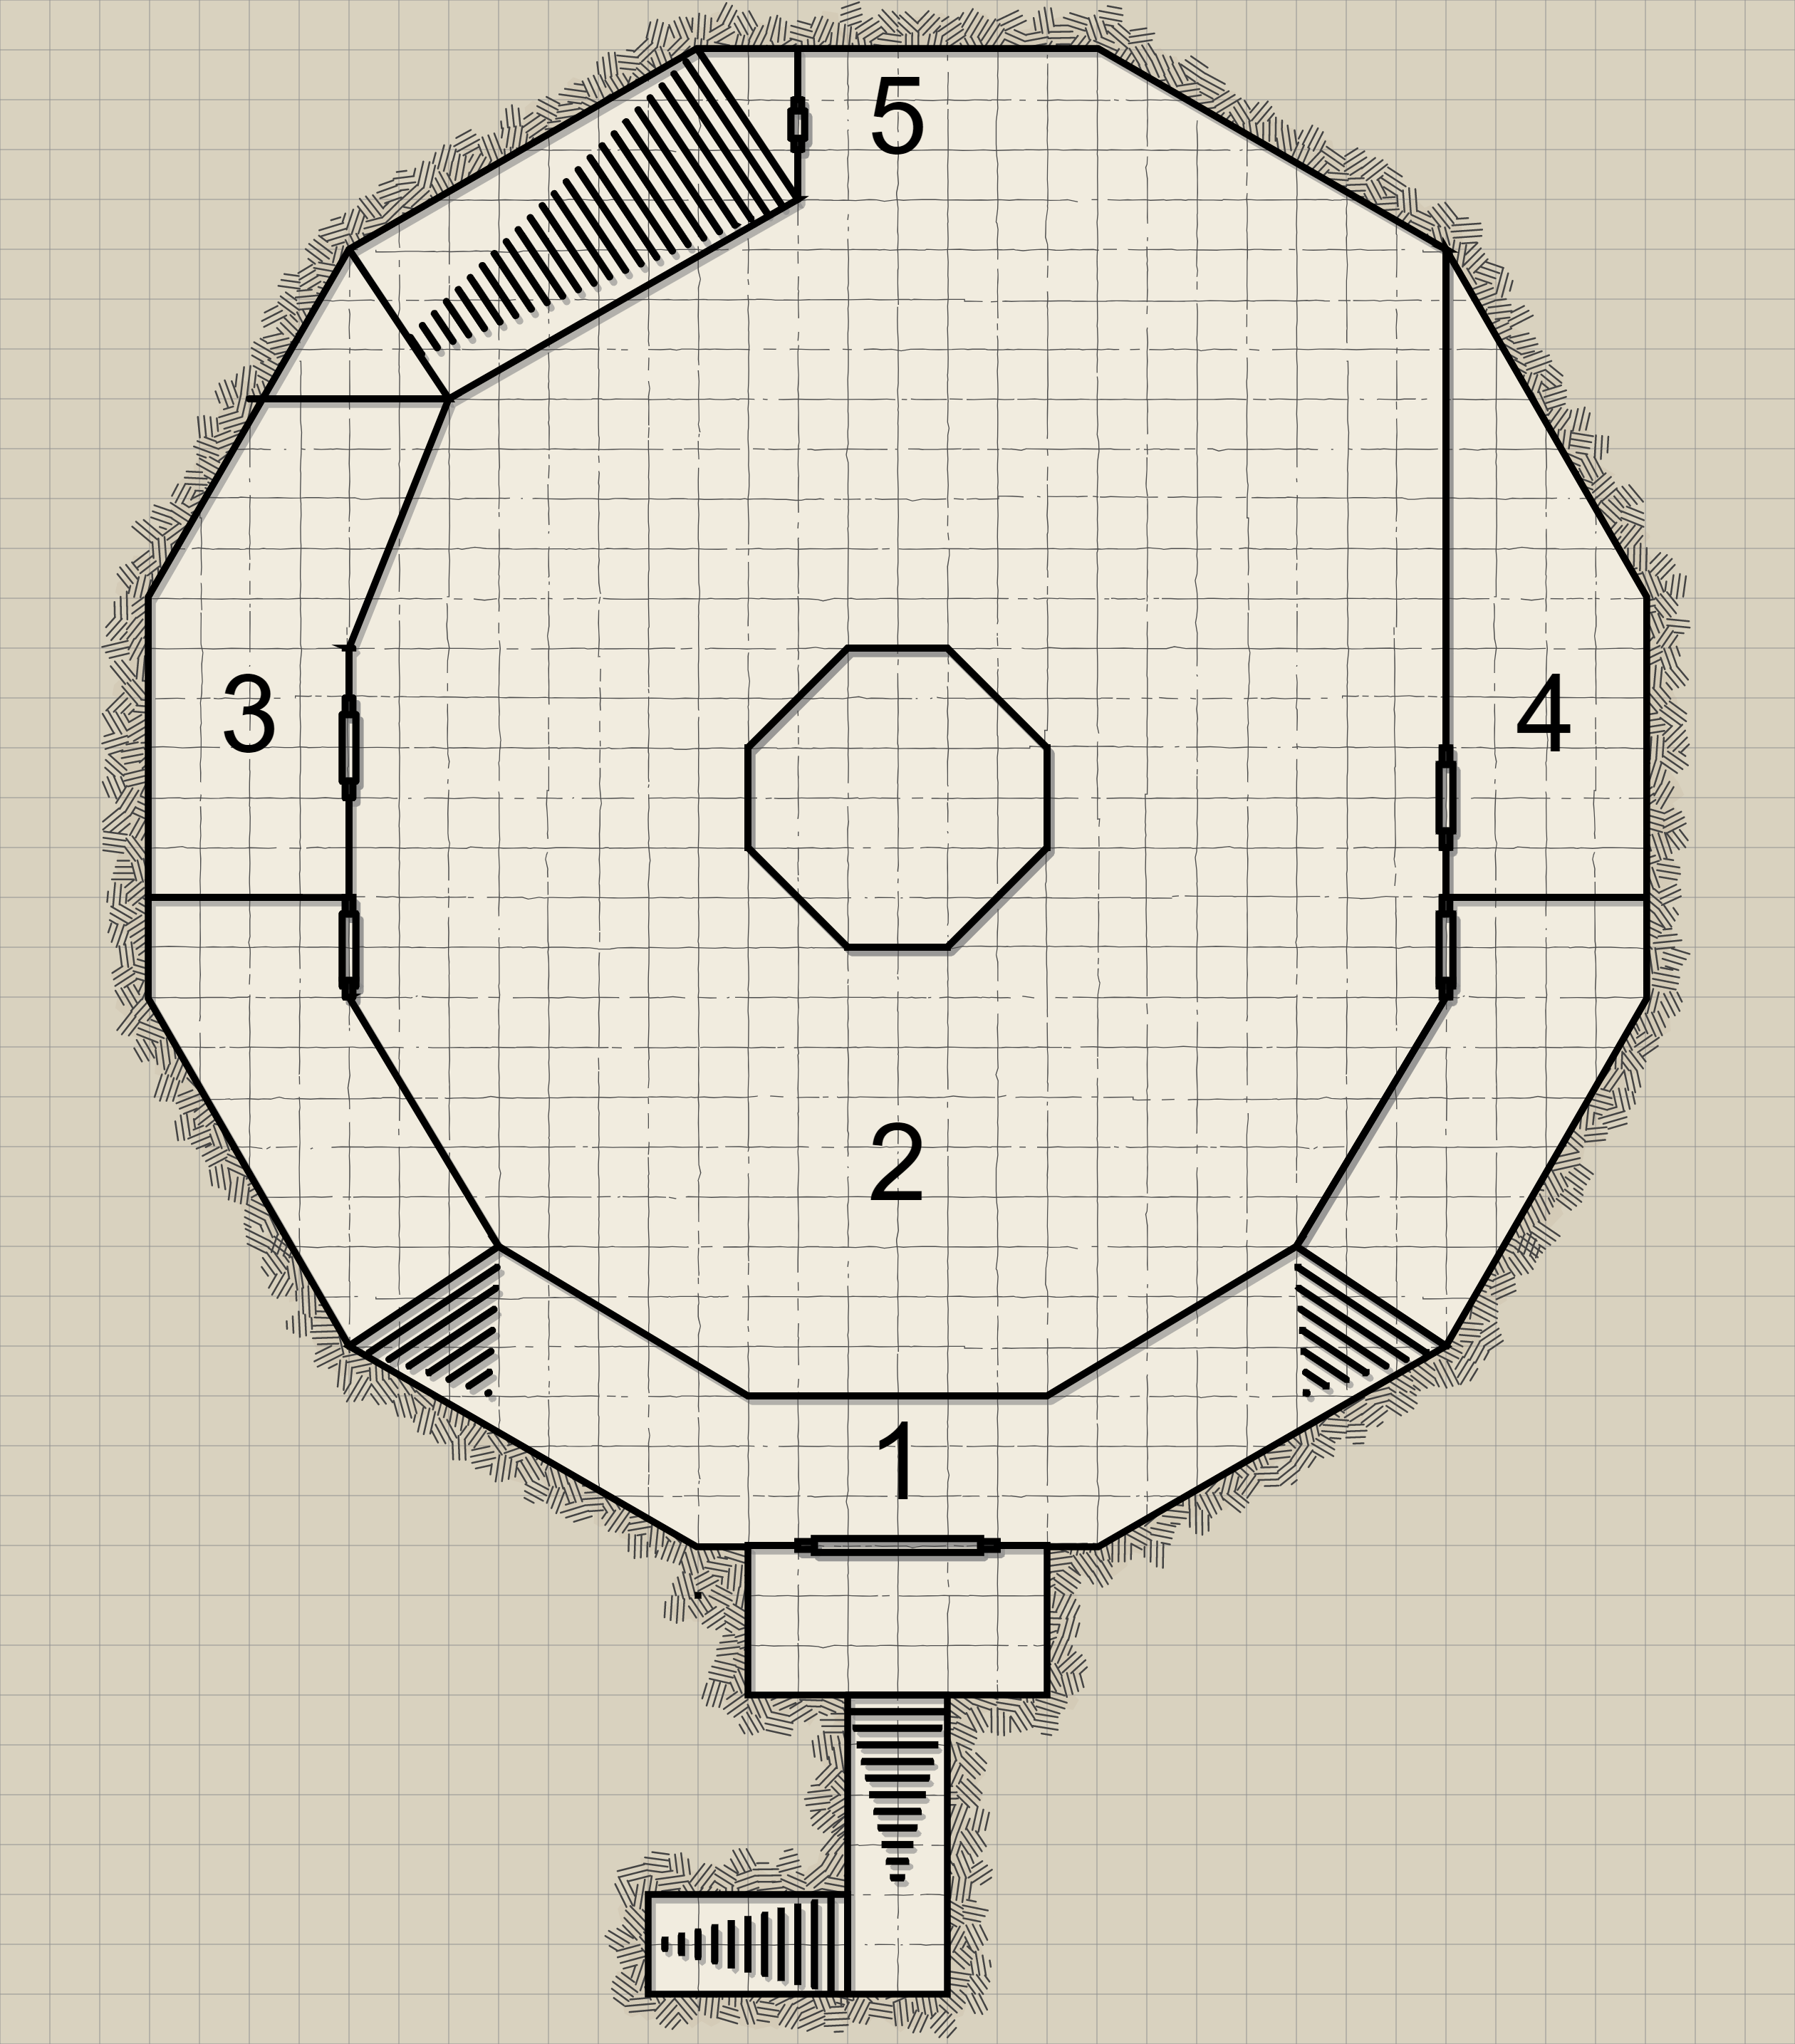
\includegraphics[width=0.4\textwidth]{images/observatory}
			\caption{The Valboro Observatory Top Level}
		\end{figure*}
	
		\subsubsection*{\underline{1. Main Entrance and Foyer}}
	
		Once the players enter the observatory, time is set at a standstill due to the rift. The observatory is normally a busy environment where scientist perform their weather research, however, this observatory has been completely abandoned for what appears to be years or decades, or even possibly longer. Trying to leave through the main doors opens up to a mirrored copy of the inside of the observatory. Going in or out of the doors always results in starting back in the main foyer of the observatory. The foyer leads to the main telescope (\emph{area 2}) on either side. There's nothing unusual about the foyer or corridors leading to the main room, other than it is abandoned. 
		
		\subsubsection*{\underline{2. Main Telescope Room}}
		The main telescope room is in complete disarray. What was once a technological marvel has now been damaged beyond repair left to rust away. The main telescope is a very large lens that appears to be pointing out into the night sky, but isn't functional. The controls to move it have been broken and rendered unusable. Debris litters the floor showing signs of a fight occurring in this room. The players may investigate the room but all that can be found are various documents and old reports which appear to have faded with time. There are three additional doors in the main room. The western door leads to \emph{area 3} which is the main laboratory. The eastern door leads to Frunsmag's office \emph{area 4}. The northern door (\emph{area 5}) has been barricaded and leads down to the ancient telescope.
		
		\subsubsection*{\underline{3. Laboratory}}
		The laboratory is not in any much better state than any of the other rooms. It contains many spilled over or abandoned experiments. The floors are covered with sharp broken glass from broken tubes and various other glass labware. Any player investigating the room require a DC 10 acrobatic check or take 1d6 slashing damage upon falling. The only object of value in this room is a \textbf{Potion of Timeless Life} but the players will need a DC 15 investigation check to find it. Unless they have found the similar vial in Frunsmag's office, identifying the potion requires a DC 15 arcana or medicine check. 
		
		\subsubsection*{\underline{4. Frunsmag's Office}}
		Frunsmag's used this office to try to find an escape from the observatory when he was still alive. The walls are covered with writings of what appears to be someone completely going mad. Most of the writing is along the lines of "NO TIME", "DEATH IS WELCOMED HERE", "ESCAPE". In the corner of the room is a bed containing the remains of Frunsmag. Investigating the body reveals it appears he died of old age, over a hundred years ago.
		
		The room contains a desk with scattered papers and Frunsmag's journal. The journal contains a log of Frunsmag's captivity in the observatory. The first few entries are dated a month back, but later entries have the date marked as unknown (apparently Frunsmag had lost track of time). The gist of the entries include Frunsmag's day to day life, various attempts to escape. One entry mentions his colleagues going down to the ancient telescope to try to find a way out and them being killed by a strange creature. The final entry in the journal reads:
		
		\colorbox{GreenYellow}{\begin{minipage}{0.4\textwidth}
				Date: Does it really matter?
				
				To whom ever reads this,
				
				It has been months, years, or decades since I last saw any daylight. There is no escaping this place. Death will be a welcomed event. I wish I had died and been buried in the mountain with Tarack and the rest of them. Barricading the door seemed wise at the time but now I wish I had just let that creature take me.
				
				Time has no meaning here. All I know and was taught doesn't apply here. My efforts to find the cause of this phenomenon have failed. I have explored every possible rational scientific explanation for this, yet I have no answer to give. Perhaps the answers lie in irrational ancient beliefs and mythologies? The answer might lie within the mountain at the ancient telescope built by our ancestors. Sadly, I am too old and weak to prove it.
				
				If you are reading this, don't waste your time (ha!) trying to find an exit. The answer lies deep in the mountain. Best of luck to you! 
				
		\end{minipage}}
		\break
		
		\subsubsection*{\underline{5. Barricaded Door}}
		The door has been barricaded and requires a DC 15 strength check to clear the debris blocking the door. A failure of on this check causes debris to fall on whomever is around for 2d6 of bludgeoning damage. The second attempt requires a DC 10 strength check and deals 1d6 on failure, and the debris is cleared completely. The door opens to a long staircase that leads to the ancient telescope, deep underground inside the mountain.
		
	\section{The Ancient Telescope}
	Once the debris has been cleared, the door in \emph{area 5} opens to a long staircase leading deep into the mountain. At the bottom of the staircase, a mile long straight dimly lit corridor leads to a closed door. The door opens to \emph{area 1} in the ancient library room. Once the players have entered into the library, they are now trapped in this room. Trying to escape through the door takes them into a copy of the library room, similar to the phenomenon occurring at the observatory's entrance.
	
	\subsubsection*{\underline{1. Ancient Library}}
	The ancient library is a large circular room which contains wall to wall bookshelves full of ancient and modern science, history, and mythology books. However, something unusual is happening in this room, gravity appears to be reversed. The room is actually upside down, the players are in fact standing on the ceiling. Knock over books cover the floor above the players heads. If they attempt to touch any of the objects, the objects react and fall down to the ceiling.
	
	In the center of the room is located the ancient telescope. The ancient telescope is essentially an 10 foot diameter shaft which was drilled straight through the mountain with lenses positioned at intervals within the shaft to provide maximal magnification. However, since the room is upside down, the shaft appears to be point down into the ceiling.  
	
	\begin{figure*}
		\centering
		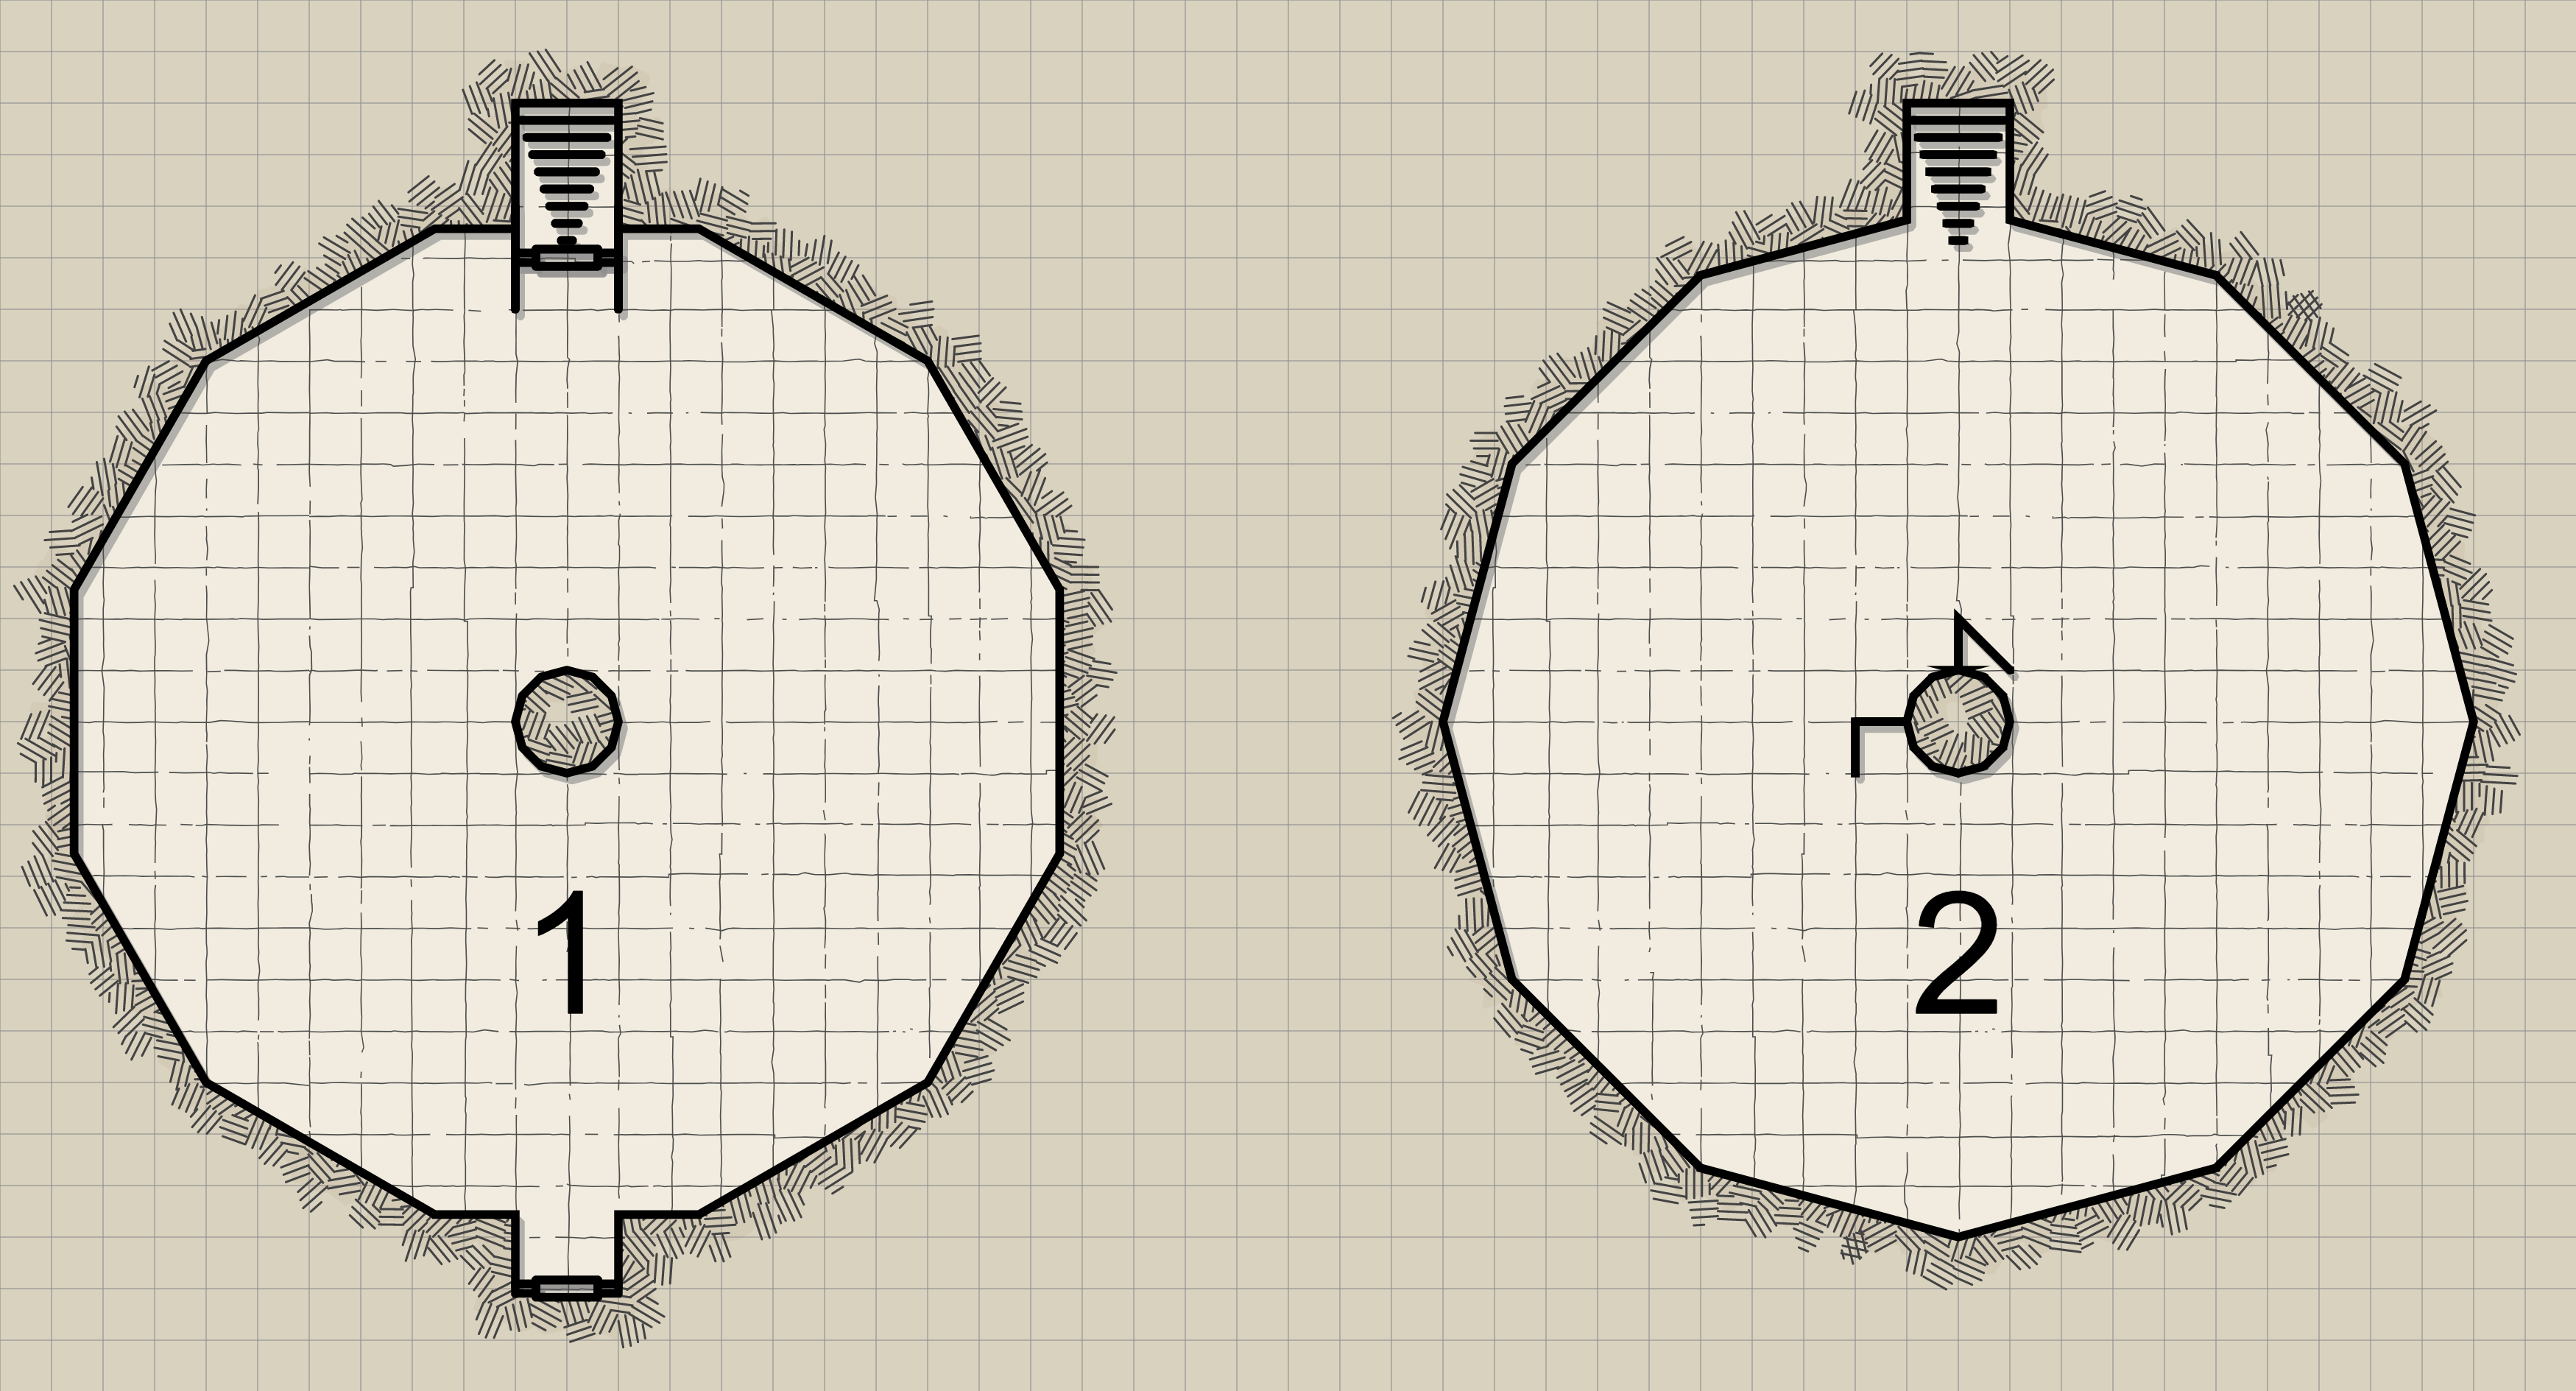
\includegraphics[width=0.8\textwidth]{images/ancient_telescope}
		\caption{The Valboro Observatory Top Level}
	\end{figure*}
	
	%\section{Treasures}

\pagebreak
	%
\section{Monsters}

\subsubsection*{Abruhani Pirates}

\subsubsection*{Child of Abruhan Cultist}

\end{multicols*}
	
\end{document}
